\documentclass[12pt,a4paper]{article}

\usepackage{fontspec}
\IfFontExistsTF{Times New Roman}
  {\setmainfont{Times New Roman}}
  {\IfFontExistsTF{CMU Serif}
    {\setmainfont{CMU Serif}}
    {\setmainfont{DejaVu Serif}}}
\IfFontExistsTF{Cascadia Mono}
  {\setmonofont{Cascadia Mono}}
  {\IfFontExistsTF{DejaVu Sans Mono}
    {\setmonofont{DejaVu Sans Mono}}
    {\setmonofont{CMU Typewriter Text}}}

\usepackage{geometry}
\geometry{left=25mm,right=15mm,top=20mm,bottom=20mm}
\setlength{\emergencystretch}{3em}
\usepackage{amsmath}
\usepackage{fvextra}
\usepackage{graphicx}
\usepackage{hyperref}
\hypersetup{hidelinks}

\title{Отчёт по задаче <<Спутники и группировки>>}
\author{Смола Артём, группа 23.Б08}
\date{}

\begin{document}
\maketitle

\section{Постановка задачи}
Даны $n$ космических аппаратов (КА) и $m$ взаимодействий между ними.
Для каждого взаимодействия задан интервал времени на общей шкале $[0, T)$.
Требуется разбить глобальный интервал на такты по 10 минут и для каждого такта получить группировки КА:
два КА относятся к одной группировке, если в данном такте они связаны цепочкой активных взаимодействий.

\section{Принцип решения}
Для каждого такта $[t, t+10)$ строится граф активных связей:
ребро между КА активно, если его интервал взаимодействия пересекается с текущим тактом.
Все интервалы трактуются как полуинтервалы вида $[\text{start}, \text{finish})$.
Если во входе задано поле \texttt{len}, дополнительно проверяется равенство
$\text{len} = \text{finish} - \text{start}$.

Группировки в такте вычисляются как компоненты связности графа.
Для поиска компонент используется DSU (система непересекающихся множеств):
\begin{enumerate}
    \item Инициализировать DSU из $n$ вершин.
    \item Для каждого активного ребра выполнить объединение его концов.
    \item После обработки всех рёбер собрать вершины по корням DSU.
\end{enumerate}

Процедура повторяется для всех тактов на интервале $[0, T)$ с шагом 10 минут.

\section{Корректность}
На каждом такте строится граф активных связей.
В него попадают ровно те рёбра, чьи интервалы пересекаются с текущим тактом.

После обработки активных рёбер DSU точно задаёт компоненты связности.
По определению задачи каждая такая компонента является группировкой КА.
Так как процедура выполняется для всех тактов, программа выдаёт корректный ответ для всей шкалы времени.

\section{Ограничения реализации}
\begin{itemize}
    \item единая семантика времени: только полуинтервалы $[\text{start}, \text{finish})$;
    \item требуется $\text{start} < \text{finish}$ для каждой связи;
    \item в формате с \texttt{len} требуется строго $\text{len} = \text{finish} - \text{start}$;
    \item если задано $T$, то для каждой связи должно выполняться $\text{finish} \le T$.
\end{itemize}

\section{Исходный код}
Исходный код программы и тестовые данные доступны в репозитории GitHub:
\url{https://github.com/artem-smola/formal_lang}.

\section{Код программы}

Код программы:

{\small
\VerbatimInput[
    fontsize=\footnotesize,
    breaklines=true,
    breakanywhere=true
]{../../Code/main.cpp}
}

\section{Демонстрация работы программы}
\subsection*{1) Входные данные}
\textbf{Рассматриваемый тест:} \texttt{test1}.

Формат входных данных:
\begin{enumerate}
    \item первая строка: $n,\,m$ или $n,\,m,\,T$;
    \item далее $m$ строк связи:
    \begin{itemize}
        \item $i\ j\ start\ finish$, или
        \item $i\ j\ len\ start\ finish$;
    \end{itemize}
    \item такт фиксирован: 10 минут.
\end{enumerate}
Где $i,j$ --- номера КА, а интервал взаимодействия всегда задаётся как полуинтервал
$[\text{start}, \text{finish})$.
Если $T$ не задано, программа берёт $T = \max(\text{finish})$ по входным связям.

{\small
\VerbatimInput[
    fontsize=\footnotesize,
    breaklines=true,
    breakanywhere=true
]{../../Code/tests/test1.in}
}

\subsection*{2) Вывод}

\begin{center}

\includegraphics[
    width=\textwidth,
    keepaspectratio
]{assets/terminal_output_test1.png}
\end{center}

\subsection*{3) Визуализация}
\textbf{Такт $[0,10)$}
\IfFileExists{../../Visualization/test1_tick_0_10.png}{
\begin{center}
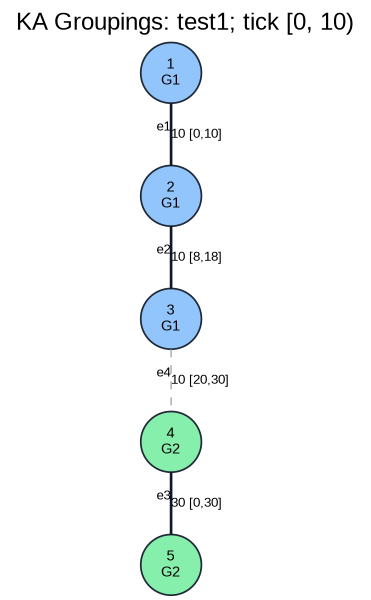
\includegraphics[
    width=\textwidth,
    height=0.30\textheight,
    keepaspectratio
]{../../Visualization/test1_tick_0_10.png}
\end{center}
}{
\textbf{Файл визуализации:} \texttt{../../Visualization/test1\_tick\_0\_10.dot}

{\small
\VerbatimInput[
    fontsize=\footnotesize,
    breaklines=true,
    breakanywhere=true
]{../../Visualization/test1_tick_0_10.dot}
}
}

\textbf{Такт $[10,20)$}
\IfFileExists{../../Visualization/test1_tick_10_20.png}{
\begin{center}
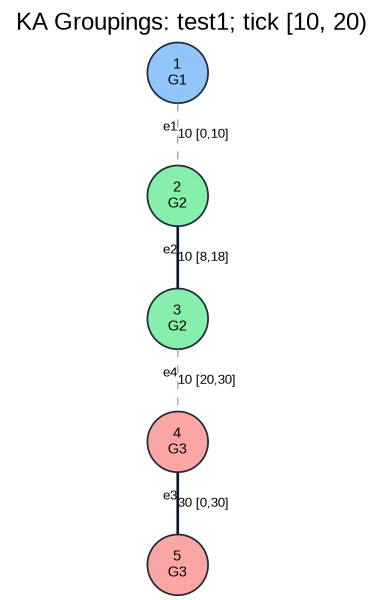
\includegraphics[
    width=\textwidth,
    height=0.30\textheight,
    keepaspectratio
]{../../Visualization/test1_tick_10_20.png}
\end{center}
}{
\textbf{Файл визуализации:} \texttt{../../Visualization/test1\_tick\_10\_20.dot}

{\small
\VerbatimInput[
    fontsize=\footnotesize,
    breaklines=true,
    breakanywhere=true
]{../../Visualization/test1_tick_10_20.dot}
}
}

\textbf{Такт $[20,30)$}
\IfFileExists{../../Visualization/test1_tick_20_30.png}{
\begin{center}
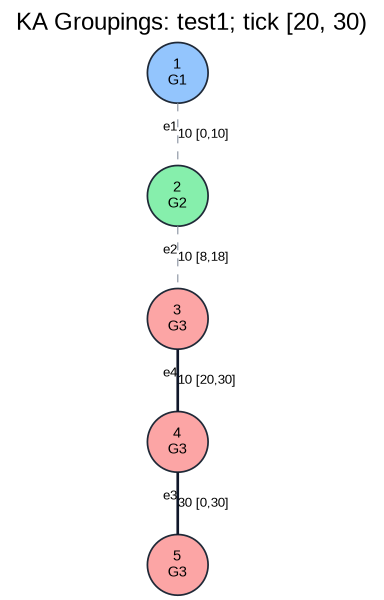
\includegraphics[
    width=\textwidth,
    height=0.30\textheight,
    keepaspectratio
]{../../Visualization/test1_tick_20_30.png}
\end{center}
}{
\textbf{Файл визуализации:} \texttt{../../Visualization/test1\_tick\_20\_30.dot}

{\small
\VerbatimInput[
    fontsize=\footnotesize,
    breaklines=true,
    breakanywhere=true
]{../../Visualization/test1_tick_20_30.dot}
}
}

\subsection*{4) Описание результата}

Для теста \texttt{test1}:
\begin{itemize}
    \item в такте $[0,10)$ формируются группы $\{1, 2, 3\}$ и $\{4, 5\}$;
    \item в такте $[10,20)$ формируются группы $\{1\}$, $\{2, 3\}$ и $\{4, 5\}$;
    \item в такте $[20,30)$ формируются группы $\{1\}$, $\{2\}$ и $\{3, 4, 5\}$.
\end{itemize}
Изменение группировок по тактам соответствует активации и деактивации интервалов взаимодействия.

\subsection*{5) Дополнительный граничный тест}
Для \texttt{test2} используется формат без явного $T$ (оно определяется как максимум $\text{finish}$),
а также несколько пересечений на границах тактов.

\textbf{Входные данные теста \texttt{test2}:}

{\small
\VerbatimInput[
    fontsize=\footnotesize,
    breaklines=true,
    breakanywhere=true
]{../../Code/tests/test2.in}
}

Результат отражает полуинтервальную семантику.
В такте $[10,20)$ формируется группировка $\{2, 3, 4, 5, 6\}$,
а КА $1$ остаётся изолированным.

\section{Анализ сложности}
Пусть $q = \lceil T / 10 \rceil$ --- число тактов.

Для каждого такта:
\begin{itemize}
    \item проверяются все $m$ связей на активность;
    \item выполняются операции DSU почти за константу (амортизированно).
\end{itemize}

Итоговая временная сложность:
\[
O(q \cdot (m + n)).
\]

Память:
\[
O(n + m)
\]
на хранение связей и структур DSU.

\end{document}
